\subsection{Problem definition}

In the last example there was a domain limited only by one side with a constant temperature at the boundary. The following problem shows the profile of a homogeneous and isotropic wall with a constant heat flow $Q_A$ on the left and a constant temperature $T_L$ on the right boundary (Fig.~\ref{fig-lhdw}). This example consists also just of diffusive heat transport.
\begin{figure}[h]
\centering
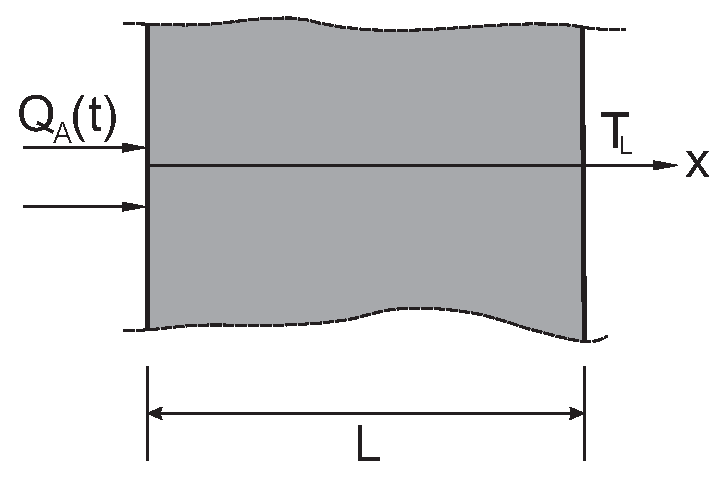
\includegraphics[width=0.5\textwidth]{T/figures/LHDW.eps}
\caption{\label{fig-lhdw}Heat conduction through a wall.}
\end{figure}
%%%%%%%%%%%%%%%%%%%%%%%%%%%%%%%%%%%%%%%%%%%%%%%%%%%%%%%%%%%%%%%%%%%%%%%%%%%%%%%%%%%%%%%%%%%%%%%%%%%%%%%%%%%%%%%%%%%%
\subsection{Analytical solution}

A solution for this problem can be found by solving the heat conduction equation \eqref{EqHT} using \textit{Fourier}'s method (see \cite{HaeSamVoi:92}). It can be shown:
\begin{equation}
\begin{split}
	T(x,t) & = T_L+\frac{Q_A}{\lambda}(L-x) + \sum_{n=1}^{\infty} \\ & - \frac{8L}{(2n-1)^2\pi^2}\;\frac{Q_A}{\lambda} \cos{\frac{(2n-1)\pi x}{2L}}\;e^{(-\frac{(2n-1)^2\pi^2}{4L^2}\alpha\,t)}
	\label{eqn:lhdw}
\end{split}
\end{equation}
with $T_L$ is the initial temperature, $Q_A$ is the constant heat source, $\lambda$ is the thermal conductivity and $\alpha$ is the heat diffusivity constant.

%%%%%%%%%%%%%%%%%%%%%%%%%%%%%%%%%%%%%%%%%%%%%%%%%%%%%%%%%%%%%%%%%%%%%%%%%%%%%%%%%%%%%%%%%%%%%%%%%%%%%%%%%%%%%%%%%%%%%%
\subsection{Numerical solution}
\subsubsection{Model setup}

The numerical model consits of 40 line elements and 41 nodes along the x-axis (Fig.~\ref{fig-mslhdw}). The step size $\Delta z$ is set to $\unit[0.1]{m}$. On the left boundary a constant source term is set. The right side obtaines a constant temperature.
\begin{figure}%[htbp]
\centering
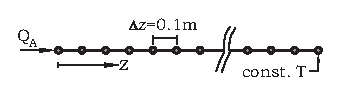
\includegraphics[width=0.5\textwidth]{T/figures/ms-lhdw.eps}
\caption{\label{fig-mslhdw}Boundary conditions and discretisation for the numerical model.}
\end{figure}

\subsubsection{Parameters}

Tab.~\ref{tab-ldhwp} shows the values of the used material properties. The heat diffusivity constant $\alpha$ 
outcomes to $\alpha = \unit[3.1 \cdot 10 ^{-6}]{m^{2}}$/s. 
\begin{table}[h]
\caption{\label{tab-ldhwp}Material properties.}
\begin{center}
\begin{tabular}{ll}
\toprule
parameter 						& value \\
\midrule
heat source $Q_A$ 				& $\unit[30]{W \cdot m^{-2}}$ \\			
initial temperatur $T_L$		& $\unit[25]{^{\circ}C}$ \\
wall thickness $L$				& $\unit[4]{m}$ \\
density of the solid $\rho$ 	& $\unit[2000]{kg \cdot m^{-3}}$ \\			
thermal capacity	$c$  		& $\unit[900]{J \cdot kg^{-1} \cdot K^{-1}}$ \\
thermal conductivity $\lambda$	& $\unit[5.5]{W \cdot m^{-1} \cdot K^{-1}}$ \\
\bottomrule
\end{tabular}
\end{center}
\end{table}

%%%%%%%%%%%%%%%%%%%%%%%%%%%%%%%%%%%%%%%%%%%%%%%%%%%%%%%%%%%%%%%%%%%%%%%%%%%%%%%%%%%%%%%%%%%%%%%%%%%%%%%%%%%%%%%%%%%%%%%
\subsection{Results}

The comparison of analytical and numerical solution is presented in Fig.~\ref{fig-lhdw-all}. The figure shows the distribution of the temperatue along the profile of the wall. Due to the thickness of the wall, the heat transport takes very long, after 5.000.000 seconds ($\approx$ 58 days) the temperature distribution becomes staedy-state.
\begin{figure}[h]
\centering
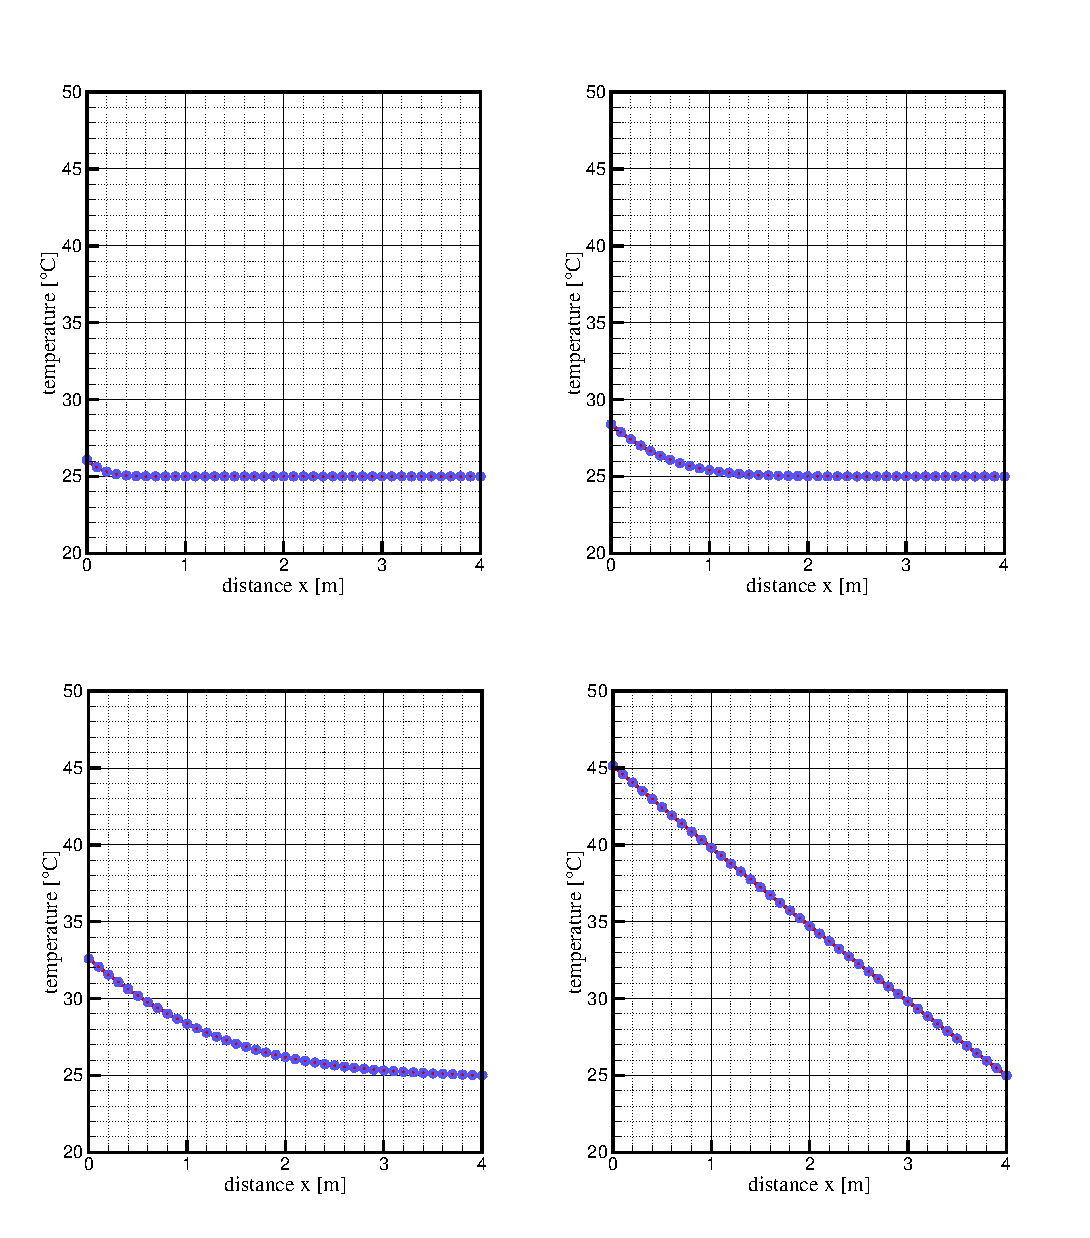
\includegraphics[width=0.8\textwidth]{T/figures/lhdw-all.eps}
\caption{Temperature distribution along the wall profile after 10.000, 100.000, 500.000 and 5.000.000 seconds (from top left to down right).}
\label{fig-lhdw-all}
\end{figure}
\begin{table}
\caption{Benchmark deposit.}
\begin{center}
\begin{tabular}{lll}
\toprule
Deposit & Version & Date \\
\midrule
T$\backslash$TDiff-wall$\backslash$TDiff-wall & 4.7.03 & Jun.~2008 \\
\bottomrule
\end{tabular}
\end{center}
\end{table}
%\clearpage